\section{Repulsive Dynamics}
\label{sec:theory}

% MANUSCRIPT-NODE: THEORY-P01
For a Gaussian policy with mean $\mu$ and covariance $\Sigma$,
\begin{equation}
\nabla_\mu\log\pi(a\mid s)=\Sigma^{-1}(a-\mu),
\label{eq:gaussian-score}
\end{equation}
so the mean-score magnitude grows with standardized distance. When covariance is learned, the variance direction depends on standardized location: the dangerous far-field chain is mean repulsion together with support contraction, not universal expansion of both mean and variance. For categorical logits $z$,
\begin{equation}
\nabla_z\log\pi(a\mid s)=e_a-\pi(\cdot\mid s).
\label{eq:categorical-score}
\end{equation}
This direct-logit score is bounded, but repeated negative updates continue to decrease the selected action's log-odds. The shared phenomenon is persistent movement toward a policy-family boundary, not an identical Euclidean gradient law.
% END-MANUSCRIPT-NODE: THEORY-P01

% MANUSCRIPT-NODE: THEORY-P02
Consider a regular minimal exponential-family policy
\begin{equation}
\pi_\eta(a)=h(a)\exp\{\eta^\top T(a)-\psi(\eta)\}.
\end{equation}
Let $p,q\ge 0$ denote aggregate positive and negative update mass, and let $\mathbf m_+$ and $\mathbf m_-$ denote their normalized sufficient-statistic moments. The population signed field is
\begin{equation}
\mathbf F(\eta)=p\mathbf m_+-q\mathbf m_--(p-q)\nabla\psi(\eta).
\label{eq:aggregate-field}
\end{equation}
These quantities define the aggregate positive--negative competition analyzed by the equilibrium theorem.
% END-MANUSCRIPT-NODE: THEORY-P02

% MANUSCRIPT-NODE: THEORY-P03
\begin{theorem}[Stable extrapolation and loss of finite equilibrium]
\label{thm:equilibrium}
Assume $p>q$ in~\eqref{eq:aggregate-field}. Define the signed target
\begin{equation}
\mathbf m^\star=\frac{p\mathbf m_+-q\mathbf m_-}{p-q}.
\label{eq:signed-target}
\end{equation}
If $\mathbf m^\star$ lies in the interior of the mean-parameter space, there is a unique finite equilibrium $\eta^\star$ satisfying $\nabla\psi(\eta^\star)=\mathbf m^\star$. Moreover,
\begin{equation}
\mathbf m^\star-\mathbf m_+=\frac{q}{p-q}(\mathbf m_+-\mathbf m_-),
\end{equation}
so negative repulsion moves the equilibrium beyond the Positive-only target in the direction away from the negative moment. As $\mathbf m^\star$ approaches the feasible boundary, the corresponding natural parameter becomes degenerate or unbounded; if the signed target lies outside the feasible mean-parameter space, no finite equilibrium exists. At an interior equilibrium, $J_F(\eta^\star)=-(p-q)\nabla^2\psi(\eta^\star)$ is negative definite.
\end{theorem}
The theorem gives one phase sequence: Positive-only, stable extrapolation, boundary approach, and loss of finite equilibrium. The experiments align this phase classification with separate measurements of task performance, policy-family boundaries, and numerical state.
% END-MANUSCRIPT-NODE: THEORY-P03

% MANUSCRIPT-NODE: THEORY-P04
Theorem~\ref{thm:equilibrium} yields direct experimental predictions. Removing negative updates should produce a stable Positive-only platform. Adding moderate negative influence should move the policy beyond that platform while retaining a finite terminal state. Increasing negative strength or outward moment should approach a covariance, support, or probability boundary; beyond the feasible region, the policy should exhibit persistent drift or a non-vanishing field residual. Finally, selective attenuation of the far-field component should restore a finite regime while retaining part of the extrapolation benefit. We test these predictions in C-U1 and D-U1, reporting task-performance collapse, support or variance boundaries, and NaN/Inf failures as separate outcomes.

\begin{figure}[t]
\centering
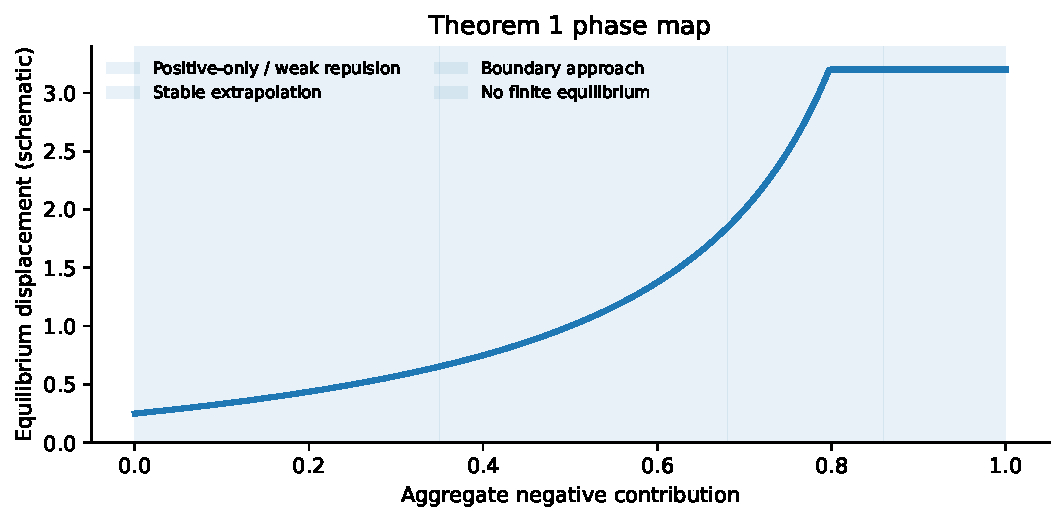
\includegraphics[width=\columnwidth]{figures/generated/fig2_phase_map.pdf}
\caption{Schematic phase map induced by Theorem~\ref{thm:equilibrium}. The empirical tests separately identify the Positive-only target, stable extrapolation, boundary approach, and persistent drift or loss of a finite equilibrium.}
\label{fig:phase-map}
\end{figure}
% END-MANUSCRIPT-NODE: THEORY-P04

% MANUSCRIPT-NODE: THEORY-P05
For Gaussian policies, an interior signed target corresponds to finite mean and covariance parameters; far-field negative updates can increase standardized displacement and contract support, causing score amplification and boundary approach. For categorical policies, an interior target corresponds to finite logits, whereas a boundary target drives selected probabilities toward zero or one. Direct-logit score norms remain bounded, but suppression persists. Thus the transferable principle is aggregate repulsion toward a feasibility boundary, while the local amplification law remains policy-family specific.
% END-MANUSCRIPT-NODE: THEORY-P05
